\documentclass{beamer}
\usepackage{listings}
\lstset{
%language=C,
frame=single, 
breaklines=true,
columns=fullflexible
}
\usepackage{subcaption}
\usepackage{url}

\usepackage{tikz}
\usepackage{pgfplots}
\pgfplotsset{compat=1.17}
\usepackage{tkz-fct}
\usepackage{mathrsfs}
\usepackage{txfonts}
\usepackage{tkz-euclide} 
\usetikzlibrary{calc,math}
\usepackage{float}
\newcommand\norm[1]{\left\lVert#1\right\rVert}
\renewcommand{\vec}[1]{\mathbf{#1}}
\providecommand{\pr}[1]{\ensuremath{\Pr\left(#1\right)}}
\usepackage[export]{adjustbox}
\usepackage[utf8]{inputenc}
\usepackage{amsmath}
\usetheme{Boadilla}
\title{Research Paper Presentation}
\author{P Ganesh Nikhil Madhav - CS20BTECH11036}

\begin{document}
\begin{frame}
\titlepage
\end{frame}
\section{}
\begin{frame}{Performance Analysis of Signal Pattern Reducing Techniques for Low probability of Detection }
\begin{block}{Abstract}
\begin{enumerate}
    \item We will talk about the communication system based on Quasi Synchronous(QS)CDMA.
    \item  Disturbing those recurring patterns can reduce the probability of detection measured in terms of the Degree of Cyclostationarity (DCS).
    \item We aim to achieve that by employing some techniques that will perturb the signal structure by randomly selecting spreading sequences, random time dithering or a combination of the two. 
    \item We study and compare the performance of all the above techniques.
\end{enumerate}

\end{block}
\end{frame}
\section{Introduction}
\begin{frame}{Keywords and some definitions}
\begin{block}{ Code Dimensional Multiple access (CDMA)}
     CDMA is an example of multiple access, where several transmitters can send information simultaneously over a single communication channel.
\end{block}
\begin{block}{Bit Error Rate (BER)}
       The BER is the number of bit errors per unit time.that can be caused due to noise,interference or bit synchronization errors
\end{block}
\end{frame}
%\begin{frame}{Keywords}
%\begin{block}{Quadrature Amplitude Modulation (QAM):}
%       It utilises both amplitude and phase components that is able to provide high levels of spectrum usage efficiency
%    \end{block}
%    \begin{block}{Phase Shift Keying (PSK):}
%       A digital modulation process which conveys data by modulating the phase of a constant frequency carrier wave.
%    \end{block}
%\end{frame}


\begin{frame}{System Model}
\begin{block}{Introduction }
\begin{enumerate}
     \item Normally in QS-DS-CDMA each user spreads all their symbols using the same (unique) spreading sequence.
\end{enumerate}
\end{block}
\begin{block}{ LS Code }
 A LS code is defined by the triplet ($M,{L}_{c},Z$)
\begin{enumerate}
     \item $M$ is Family Size.
     \item $L_{c}$ is code length.
     \item  $Z$ is the size of the code’s ZCZ.
     \item Fundamental orthogonal bond ,i.e $L_{c} = M.Z$
\end{enumerate}
\end{block}
\end{frame}


\begin{frame}{System Model}
\begin{block}{The transmitted signal  model}
    The transmitted signal of a user in a Quasi Synchronous (QS)-DS-CDMA system is modeled as
\begin{align}
    x(t)& = \sum_{n = 0}^{N-1}b_{n}\sum_{l= 0}^{L-1}a_{l}p(t - lT_{c} -nT - \Delta t)
    \label{eq1}
\end{align}
spreading sequence is $\{a_{0},a_{1},.....a_{L-1}\}$ of length L
\end{block}
\end{frame}

\begin{frame}{System Model}
\begin{block}{Parameters}
\begin{table}[]
\centering
\renewcommand{\arraystretch}{1.4}
\begin{tabular}{|c|c|}
        \hline
        Parameter& Parameter Denotes \\ \hline
        $N$ & Number of data symbols transmitted per packet\\ \hline
        $T$ & Symbol duration\\ \hline
        $b_{n}$ &  The nth symbol which is spread by  sequence of length $L$\\ \hline
        $T_{c}$ & Chip duration \\ \hline
        $\Delta t$ & Time uncertainty due to imperfect synchronization \\ \hline
\end{tabular}
\caption{Parameters}
\label{tab:my_label}
\end{table}
\end{block}
    
\end{frame}


\begin{frame}{Pattern Reducing Schemes}
\begin{block}{Pattern Reducing Schemes : }
\begin{enumerate}
    \item Random Spreading Sequence Selection (RS-MECS).
    \item Random Time Dithering (DITH).
    \item Random Selection with Dithering (RS-DITH).
\end{enumerate}
\end{block}
\end{frame}

\begin{frame}{Random Spreading Sequence Selection}
    \begin{block}{RS-MECS}
    In this , we describe and analyze a scheme for spreading sequence assignment and random selection which we call Random Selection from Mutually Exclusive Code Subsets (RS-MECS).
\begin{enumerate}
    \item In this scheme, We instead propose a system where each user is assigned a set of sequences; spreading is then performed by picking one of those sequences randomly in a per-symbol basis.
\end{enumerate}
    \end{block}
    \begin{block}{Note}
     It is not necessary to make a ‘symmetric’ sequence assignment, as shown in the following example.
    \end{block}
\end{frame}

\begin{frame}{Example for RS-MECS}
\begin{figure}
    \centering
    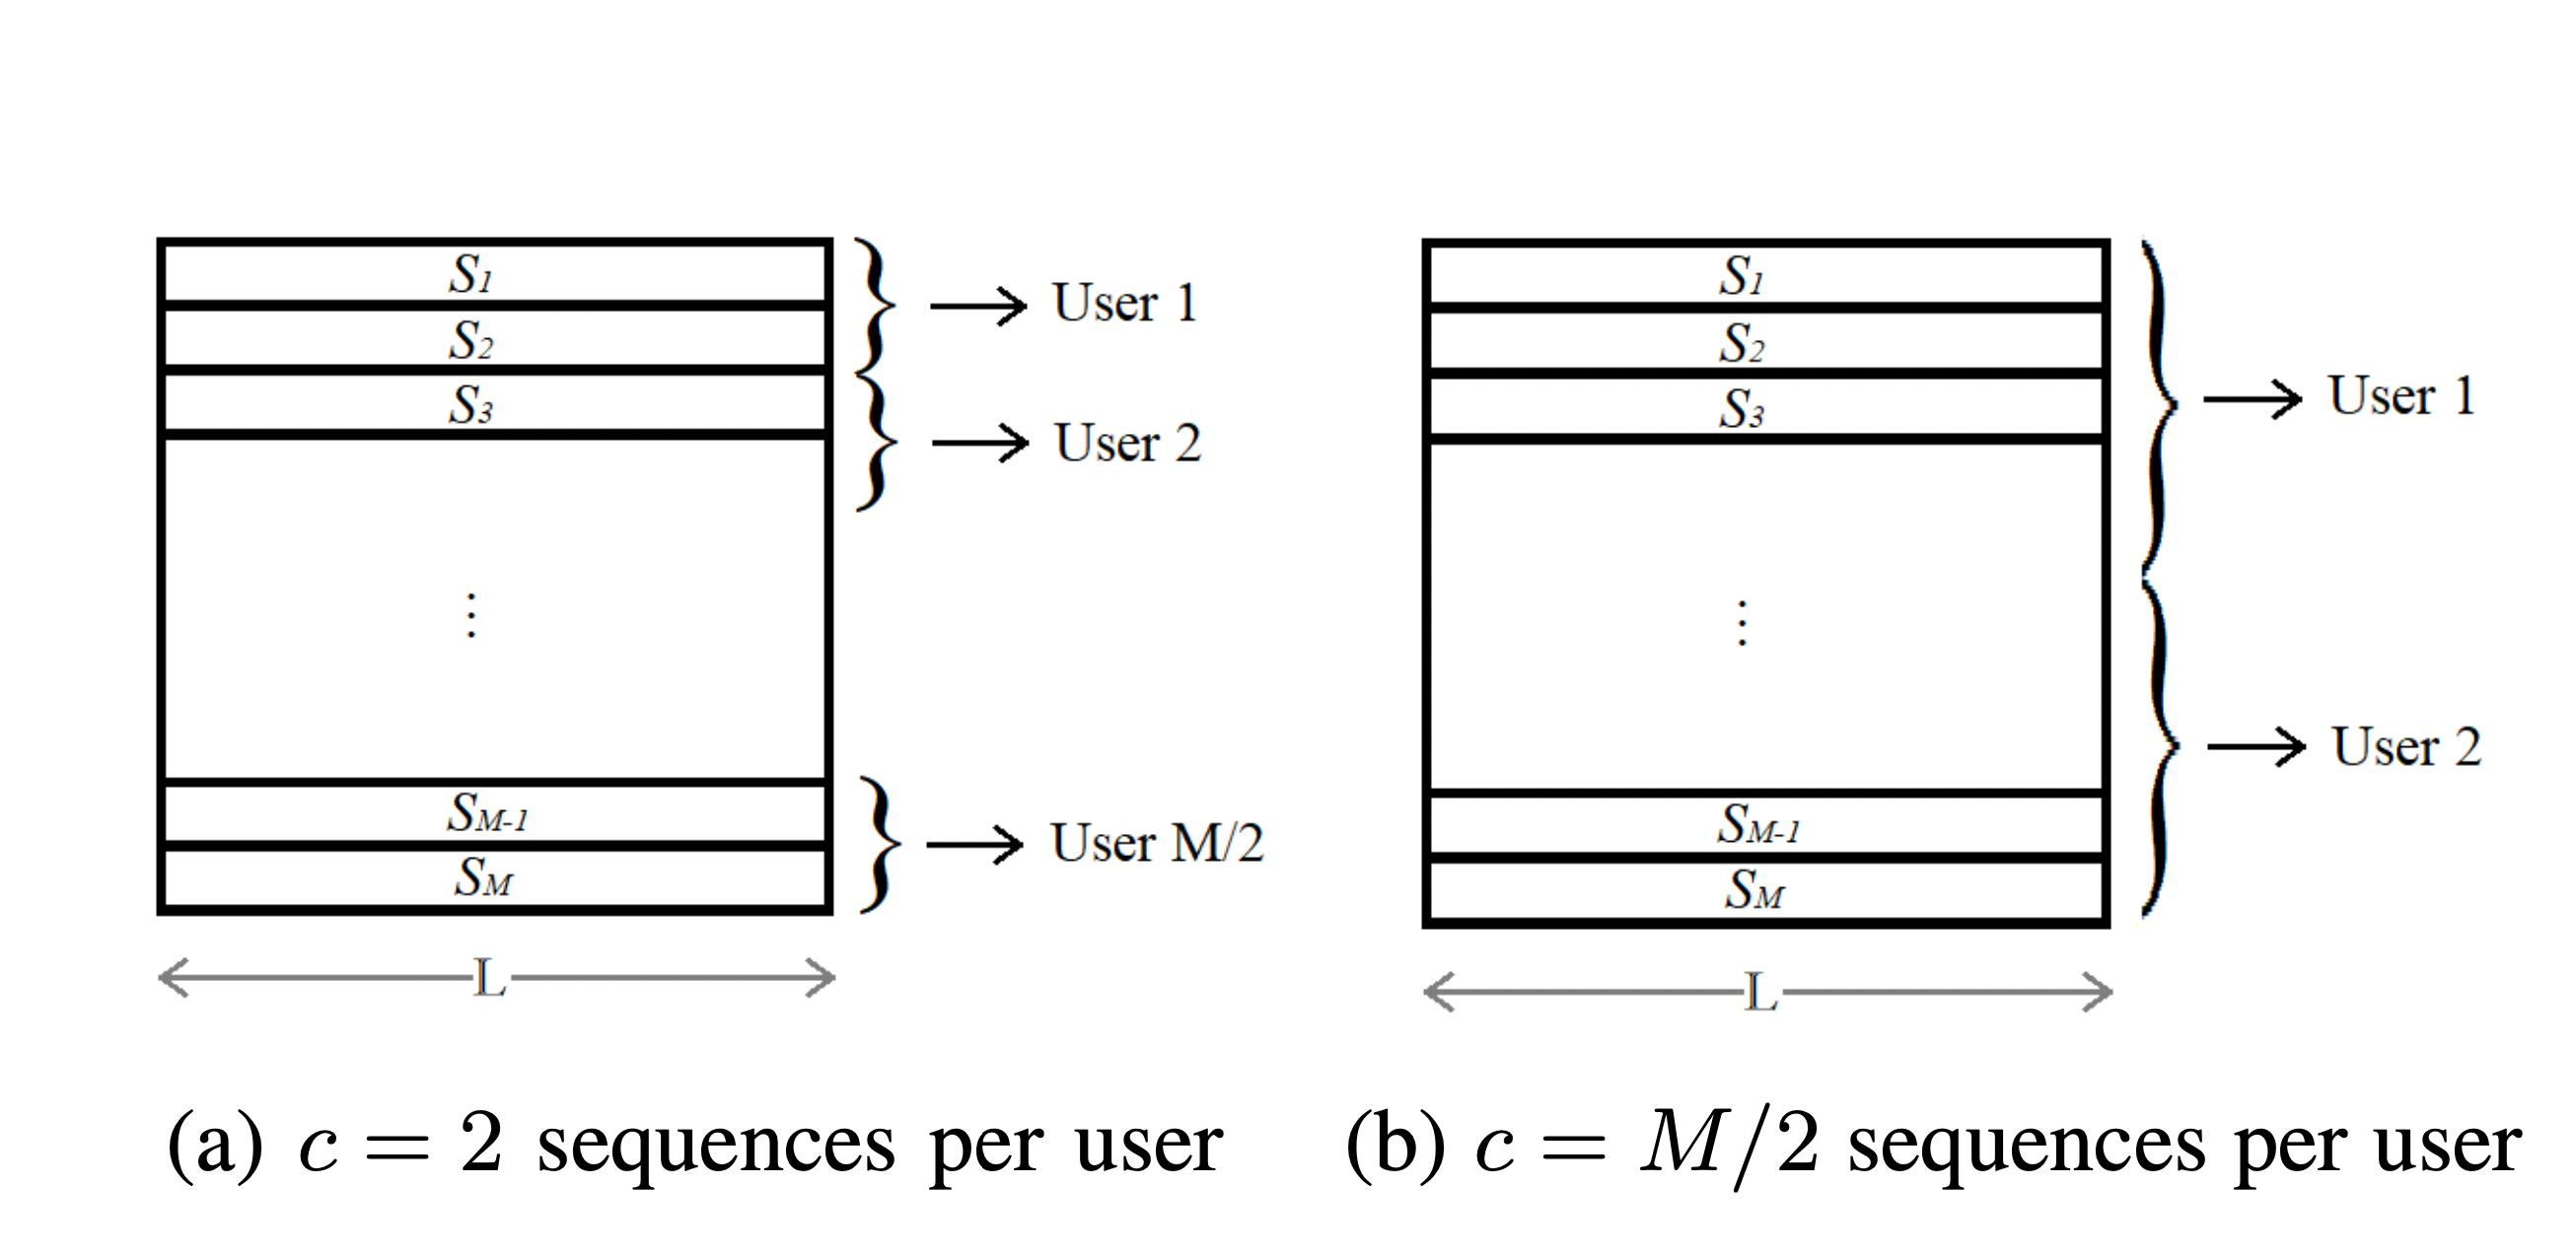
\includegraphics[width=0.6\columnwidth]{Examples of RS-MECS.png}
    \caption{RS-MECS Examples}
    \label{fig:1}
\end{figure}
\end{frame}

\begin{frame}{Random Spreading Sequence Selection}
\begin{block}{The transmitted signal model}
   The transmitted signal model then becomes
\begin{align}
    x(t)& = \sum_{n = 0}^{N-1}b_{n}\sum_{l= 0}^{L-1}a_{l,n}p(t - lT_{c} -nT - \Delta t)
    \label{eq2}
\end{align}
   In this case , Spreading sequence is additionally indexed by data symbol number ,When compared to equation \eqref{eq1};
\end{block}
\end{frame}




\begin{frame}{Random Time Dithering}
\begin{block}{DITH}
\begin{enumerate}
    \item In this technique each user is assigned a unique sequence to spread their data.
    \item Given the time uncertainty requirement of the
system, one could choose a longer ZCZ i.e Z than the one required for weak synchronization in order to introduce an additional random delay (dither)
\end{enumerate}
\end{block}

\end{frame}

\begin{frame}{Random Time Dithering}
\begin{block}{The transmitted signal model}
The transmitted signal model then becomes
\begin{align}
    x(t)& = \sum_{n = 0}^{N-1}b_{n}\sum_{l= 0}^{L-1}a_{l}p(t - lT_{c} -nT - \Delta t -\epsilon_{n} T_{c})
    \label{eq3}
\end{align}
   In this case ,Additional Term ($\epsilon_{n} T_{c}$)  accounts for random time dithering on a per-symbol basis. When compared to \eqref{eq1} ;
\end{block}
    
\end{frame}

\begin{frame}{Random Selection with Dithering}
\begin{block}{RS-DITH}
    In this scheme, that we will refer to as Random Selection with Dithering (RS-DITH), each user is assigned a set of spreading sequences and is also allowed to perform dithering within the ZCZ .
\end{block}
\begin{block}{The transmitted signal model}
   The transmitted signal model then becomes
\begin{align}
    x(t)& = \sum_{n = 0}^{N-1}b_{n}\sum_{l= 0}^{L-1}a_{l,n}p(t - lT_{c} -nT - \Delta t -\epsilon_{n} T_{c})
    \label{eq4}
\end{align}
   In this case ,both dithering and a symbol-dependent terms get included, When compared to \eqref{eq1} ;
\end{block}
\end{frame}
\begin{frame}{Auto correlation function (ACF)}
\begin{block}{ACF}
    The autocorrelation function is the correlation between the random variables corresponding to two time instants of the random signal,or
    \begin{align}
            R_{x}(t_{1},t_{2}) & = E[x(t_{1}).x^{*}(t_{2})]
    \end{align}
    To see how the autocorrelation varies with some particular central time $t$, we can use a more convenient parameterization of the two time instants $t_{1}$ and $t_{2}$, such as
    \begin{align}
    R_{x}(t,\tau) & = E[x(t + \tau/2).x^{*}(t - \tau/{2})]
    \end{align}
\end{block}
\end{frame}



\begin{frame}{LPD Evaluation - Cyclic Spectral Analysis}
\begin{block}{LPD }
    Cyclostationary signals have either a periodic or an almost periodic autocorrelation function which, for a signal $x(t)$, can be represented by a Fourier series as
\begin{align}
    R_{x}(t,\tau) & =\sum_{\alpha} R_{x}^{\alpha}(\tau)e^{i2\pi\alpha t}
    \label{eq5}
\end{align}
    The coefficient $R_{x}^{\alpha}(\tau)$ is Cyclic Autocorrelation Function (CAF)
\begin{align}
    R_{x}^{\alpha}(\tau) & =\lim_{T \to \ \infty} \int_{-T/2}^{T/2}x(t - \tau /2)x^{*}(t + \tau /2)e^{-i2\pi\alpha t} dt
    \label{eq6}
\end{align}
\end{block}
\end{frame}

\begin{frame}{LPD}
\begin{block}{Parameters}
\begin{table}[]
\centering
\renewcommand{\arraystretch}{1.4}
\begin{tabular}{|c|c|}
        \hline
        Parameter& Parameter Denotes \\ \hline
        $\tau$ & lag parameter \\ \hline
        $\alpha$ & Cycle frequency\\ \hline
        T & fundamental period of signal \\ \hline
\end{tabular}
\caption{Parameters}
\label{tab:my_label1}
\end{table}
\end{block}
\end{frame}



\begin{frame}{LPD Evaluation }
\begin{block}{DCS}
        DCS ,Which can be computed either in time or frequency domain.Here we will compute using time domain.By Defining temporal coreal coefficient as
\begin{align}
     \gamma_{x}^{\alpha}(\tau) & = \frac{R_{x}^{\alpha}(\tau)}{R_{x}(0)}
     \label{eq7}
\end{align}
we can then write time decomposed degree of cyclostationarity as
\begin{align}
    DCS_{\tau}^{\alpha} & = |\gamma_{x}^{\alpha}(\tau)|^{2} 
   \label{eq8}
\end{align}
\end{block}
\end{frame}

\begin{frame}{LPD Evaluation }
\begin{block}{DCS}
    Frequency decomposed degree of cyclostationarity as
\begin{align}
    DCS^{\alpha} & = \frac{\int_{-\infty}^{\infty} DCS_{\tau}^{\alpha} d\tau}{\int_{-\infty}^{\infty} DCS_{\tau}^{0} d\tau}
    \label{eq9}
\end{align}
    Signal's degree of cyclostationarity over all values of $ \alpha $
    as
\begin{align}
    DCS & = \sum_{\alpha \neq 0}DCS^{\alpha}
    \label{eq10}
\end{align}
     We  define DCS ratio ,which will help in computing DCS Reduction, as
\begin{align}
    \text{DCS ratio }&= \frac{DCS \text { of signal using selected technique }}{DCS \text{ of original signal} }
    \label{eq11}
\end{align}
\end{block}
\end{frame}


\begin{frame}{Bit Error Rate(BER)}
\begin{block}{BER}
\begin{enumerate}
    \item Communication performance is measured in terms of Bit Error Rate (BER) for various values of signal to noise ratio (SNR).
    \item We introduce additive white Gaussian noise(AWGN) of various power levels . 
\end{enumerate}
\end{block}
\end{frame}


\begin{frame}{Simulation and Results}
\begin{block}{Parameters}
\begin{table}[]
\centering
\renewcommand{\arraystretch}{1.4}
\begin{tabular}{|c|c|c|c|}
        \hline
        Scheme& RS-MECS & DITH & RS-DITH \\ \hline
        $C$ & $1\leq C \leq 32$& $C =1$ & $1\leq C \leq 32$ \\ \hline
        $D$ & $D =0$ & $0 \leq D \leq 32$ & $0 \leq D \leq 32$ \\ \hline
        $L_{c}$ & 64 & 64 & 64\\ \hline
\end{tabular}
\caption{Simulation Parameters}
\label{tab:my_label2}
\end{table}
\end{block}
\end{frame}


\begin{frame}{DCS Reduction for RS-MECS and RS-DITH}
\begin{figure}
    \centering
    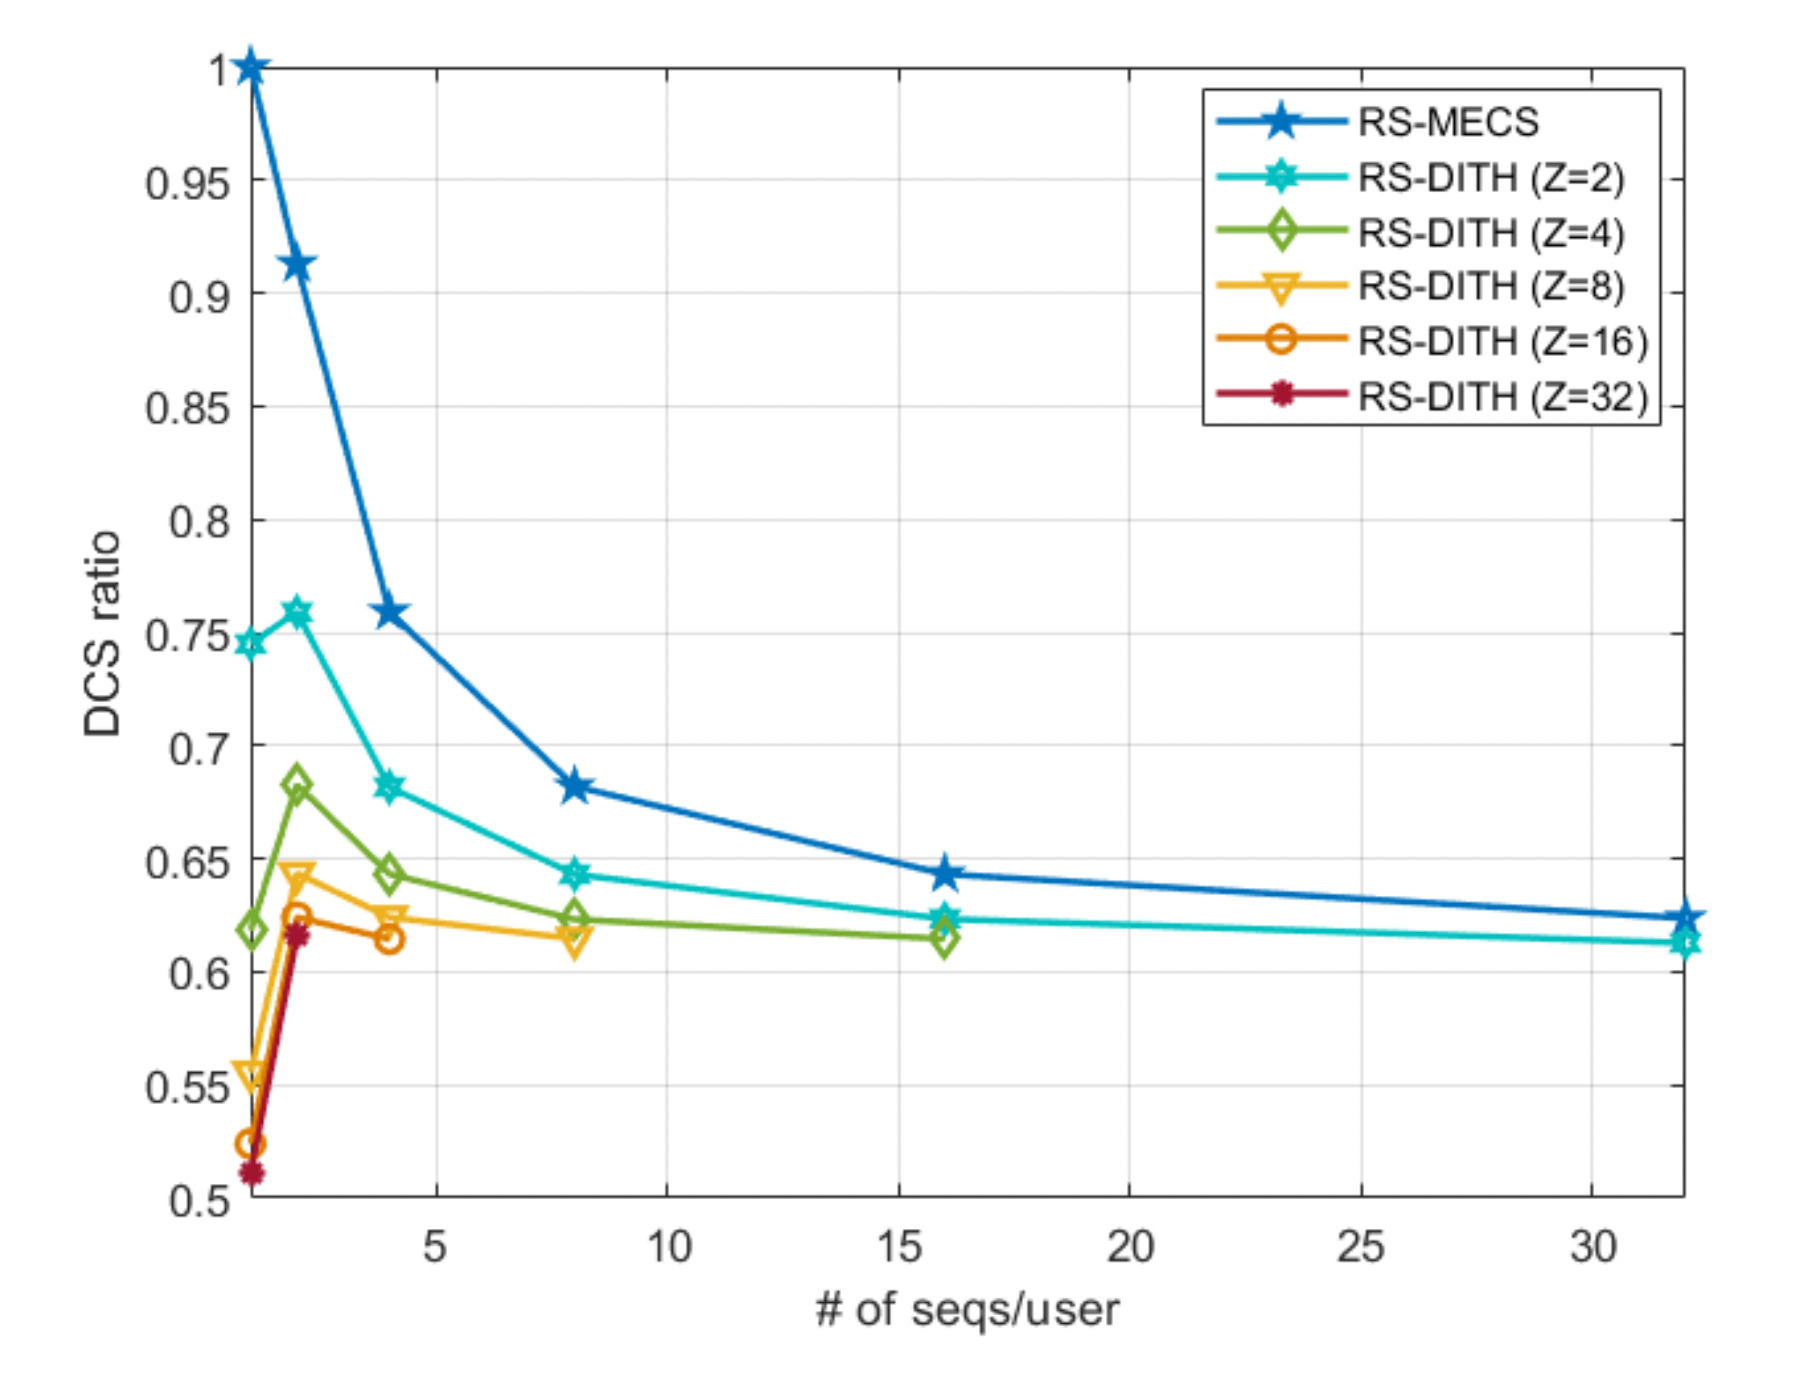
\includegraphics[width=0.6\columnwidth]{DCS ratio.png}
    \caption{DCS Reduction for RS-MECS and RS-DITH}
    \label{fig:DCS reduction for RS-MECS,RS-DITH}
\end{figure}
\end{frame}

\begin{frame}{ Results}
\begin{block}{Results}
From  Figure \ref{fig:DCS reduction for RS-MECS,RS-DITH} :
\begin{enumerate}
    \item  RS-MECS,The DCS reduction depends only on number of sequences assigned for each user,C.
    \item  RS-DITH achieves higher DCS reduction for codes with longer ZCZ and performs better than RS-MECS for a fixed value of C .
\end{enumerate}
\end{block}
\end{frame}



\begin{frame}{BER Performance of DITH, RS-MECS and RS-DITH}
\begin{figure}
    \centering
    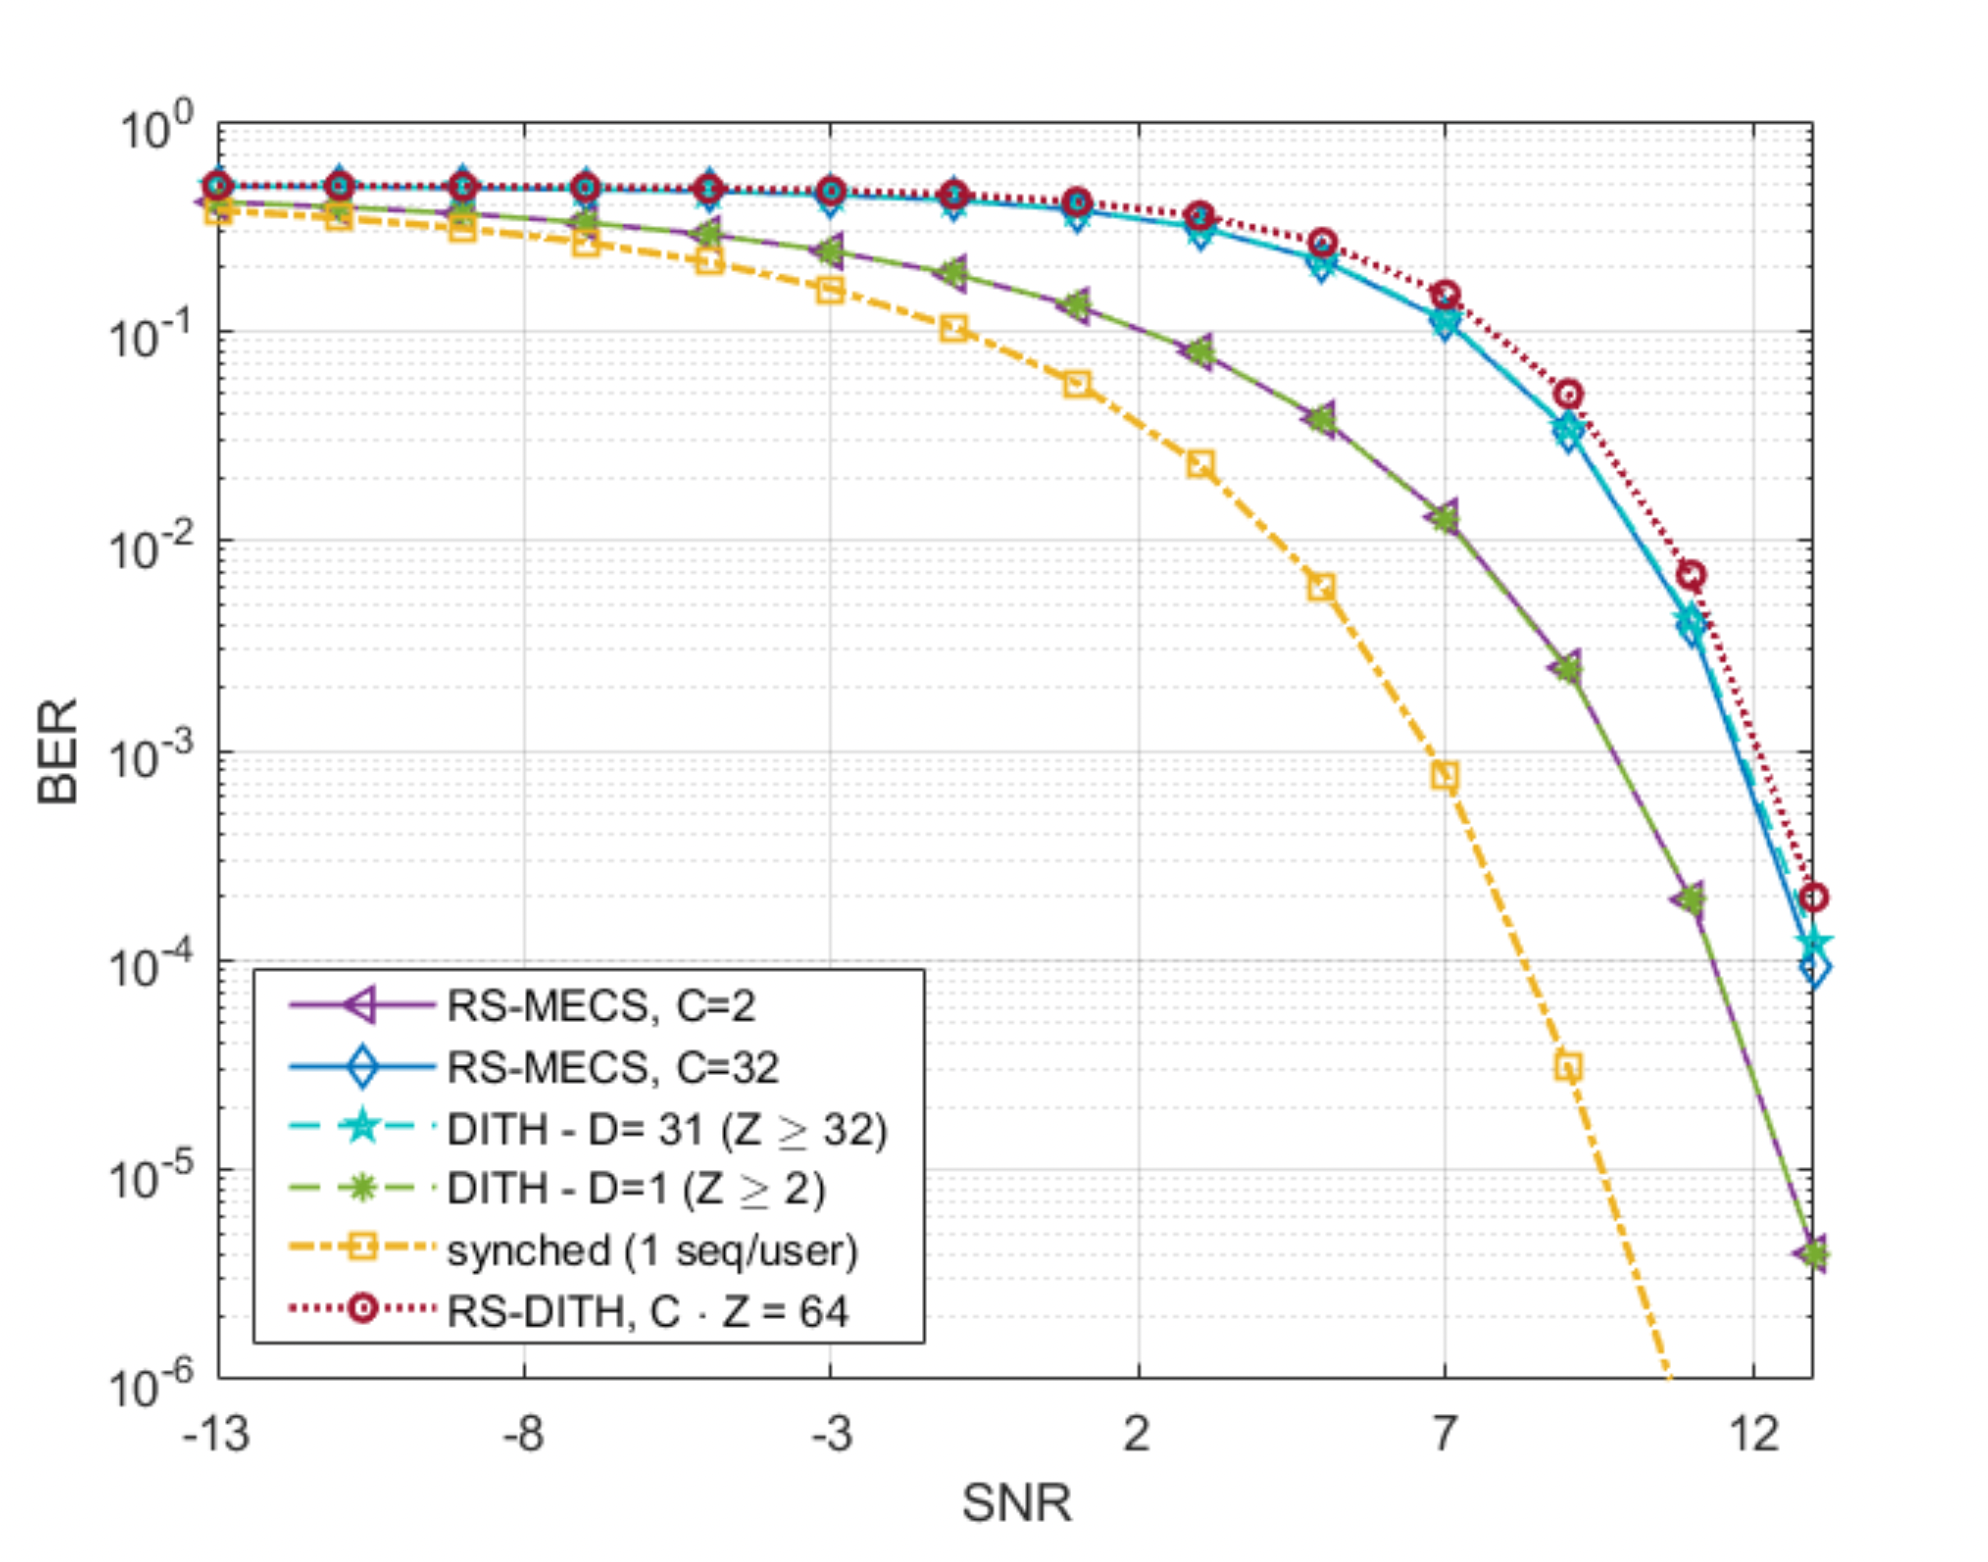
\includegraphics[width=0.6\columnwidth]{SNR vs BER.png}
    \caption{SNR vs BER Performance of DITH, RS-MECS and RS-DITH}
    \label{fig:SNR vs BER perfomance for all schemes}
\end{figure}
\end{frame}

\begin{frame}{ Results}
\begin{block}{Results}
From Figure \ref{fig:SNR vs BER perfomance for all schemes} :
\begin{enumerate}
    \item BER curves of DITH when only 1 chip of dithering is allowed coincides with BER curves of RS-MECS,when utilizing 2 sequences per user.
    \item The BER performance of RS-DITH is lower than both DITH and RS-MECS for the same codes and depends on the product $C.Z$.
\end{enumerate}
\end{block}
\end{frame}


\begin{frame}{parameters}
\begin{figure}
    \centering
    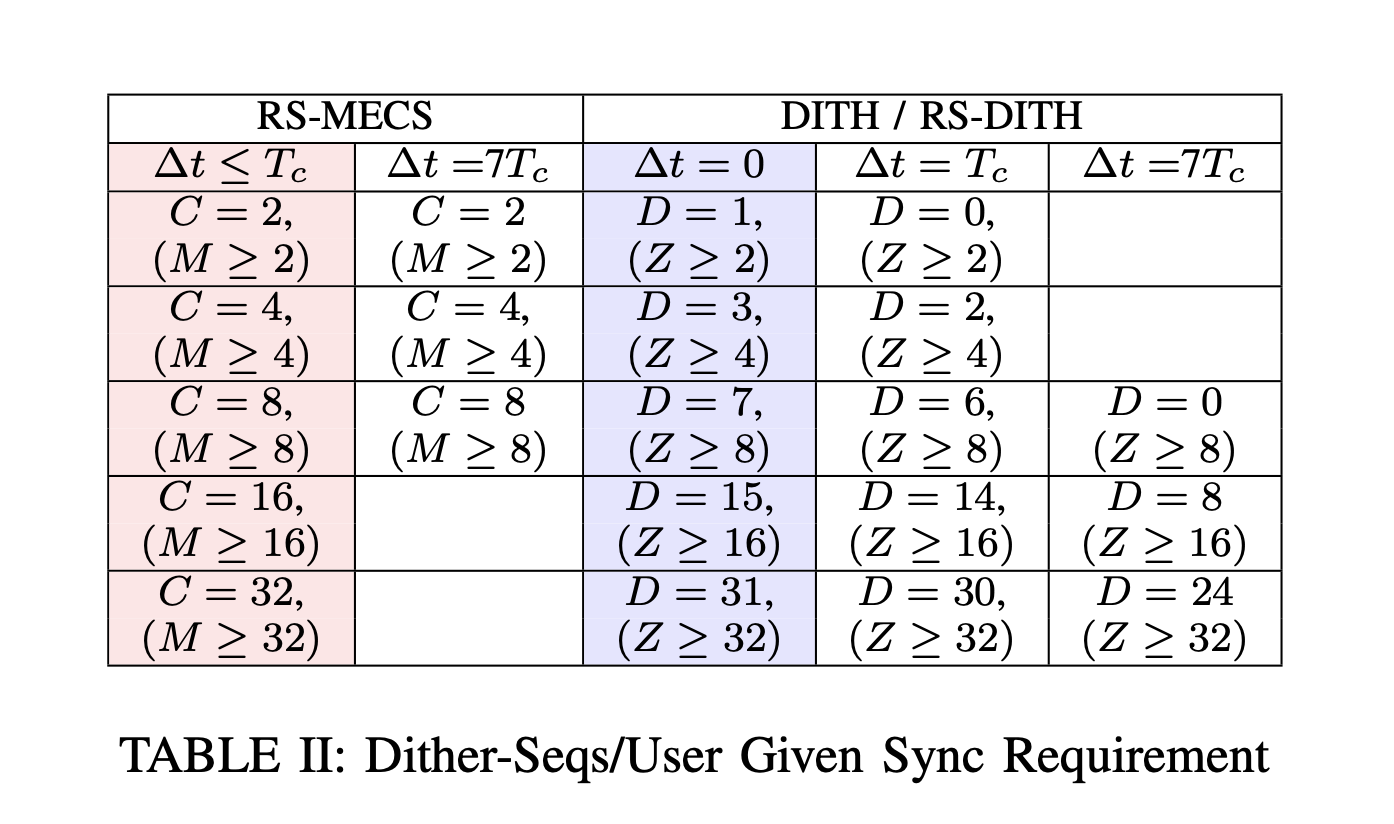
\includegraphics[width=1.0\columnwidth]{Table 2.png}
    \label{fig:Table}
\end{figure}
\end{frame}

\begin{frame}{DCS / BER Trade-off for DITH and RS-MECS}
\begin{figure}
    \centering
    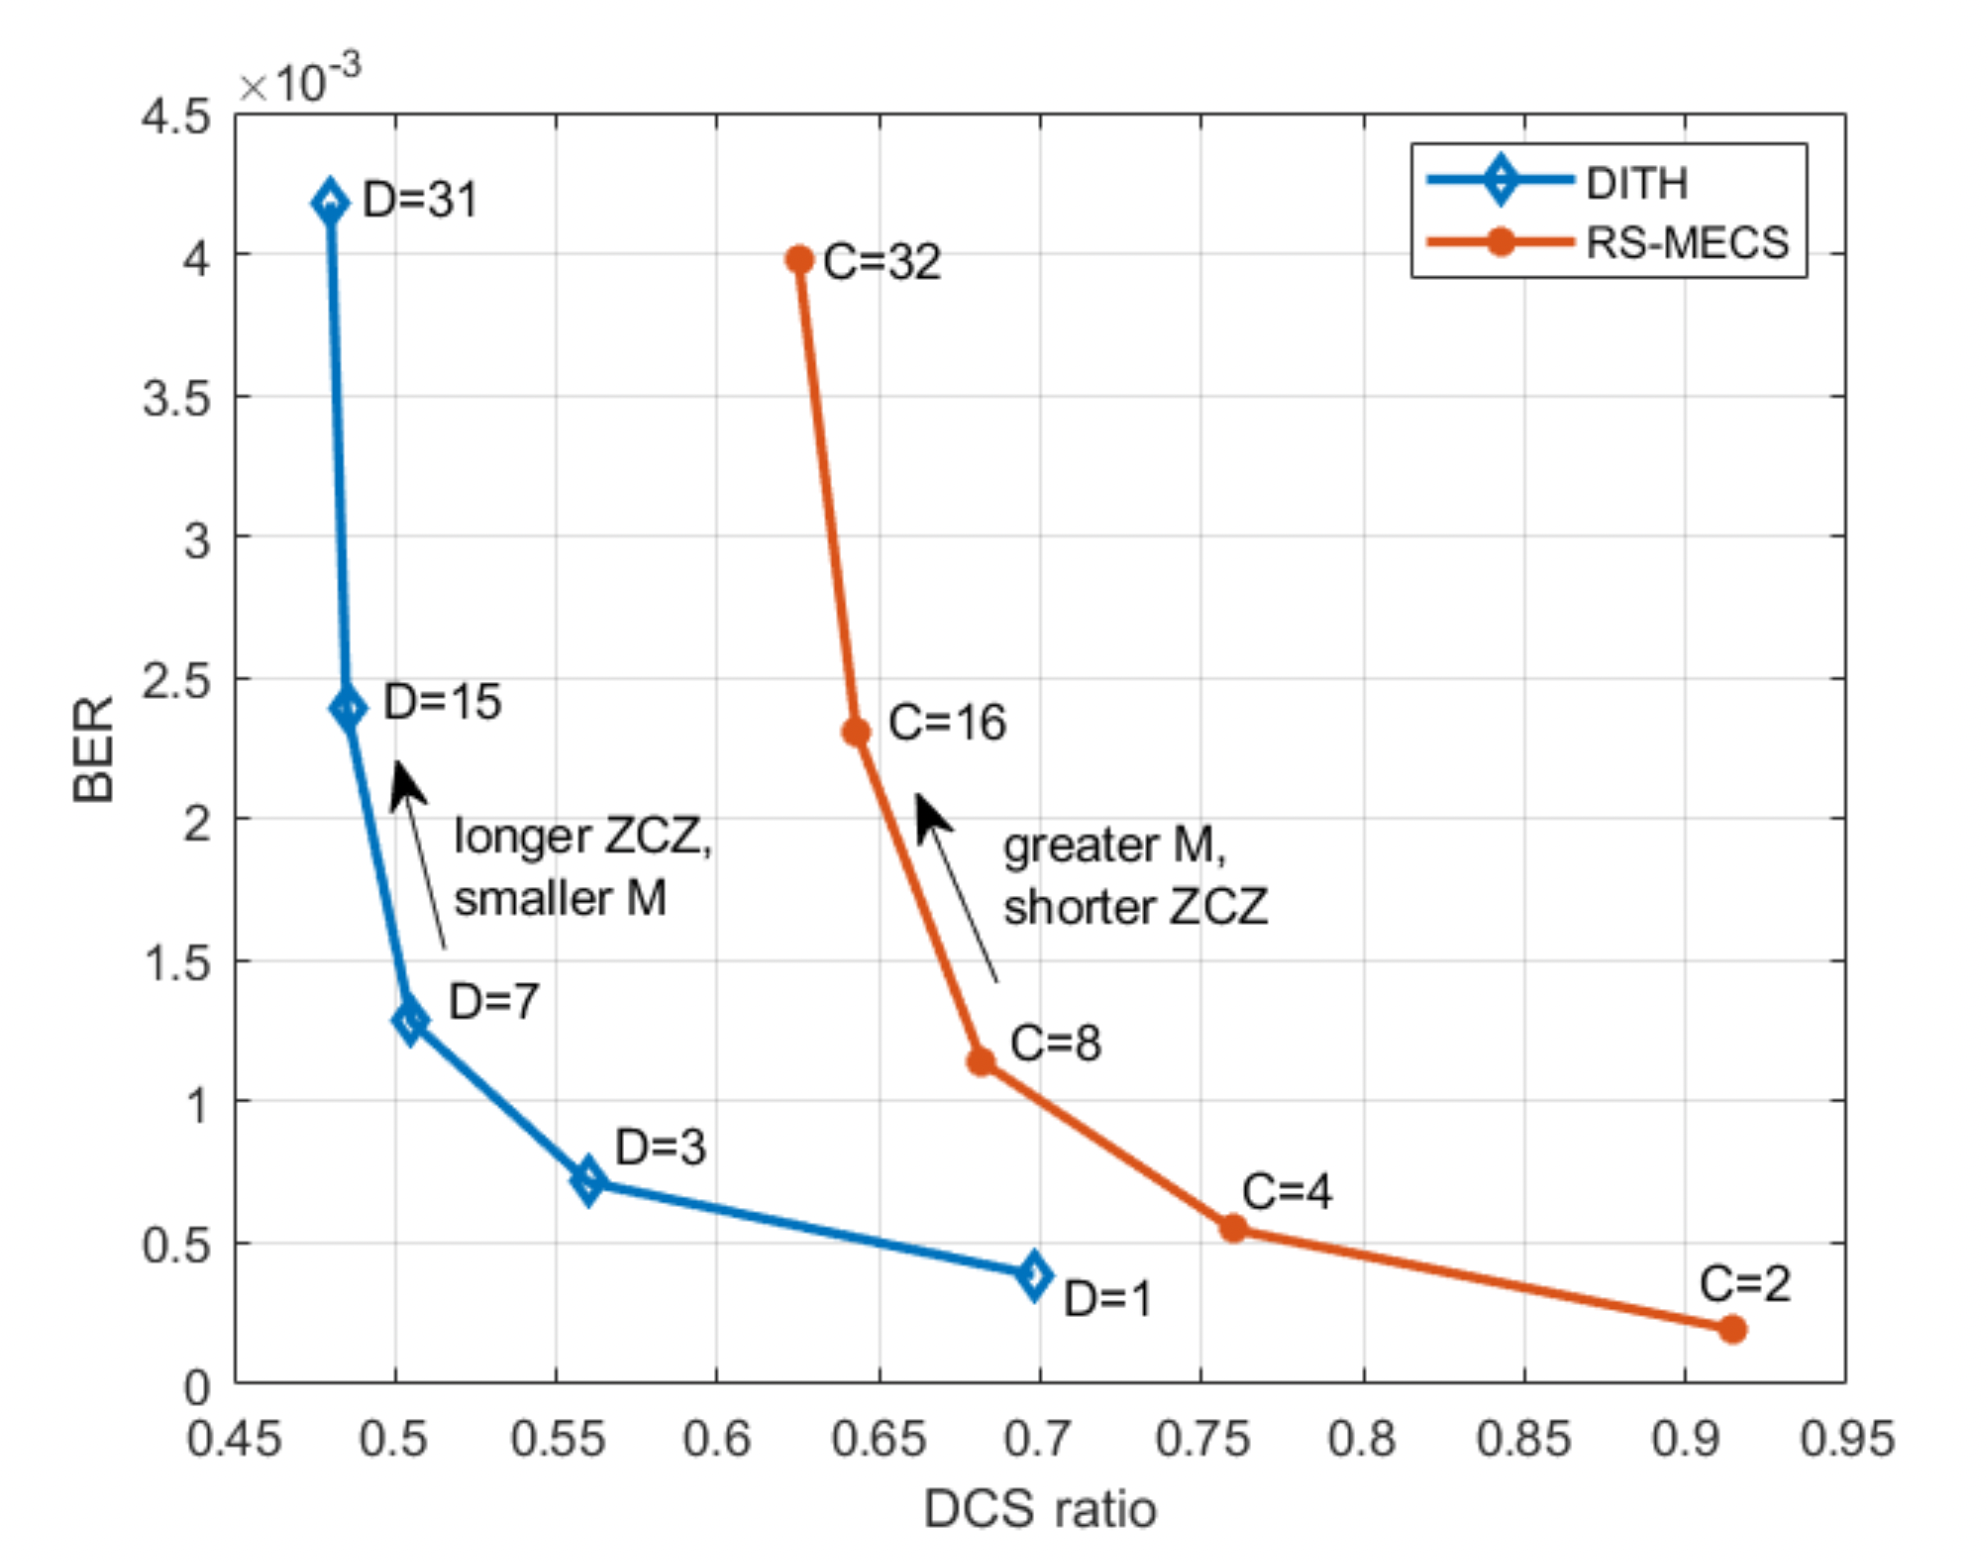
\includegraphics[width=0.6\columnwidth]{DCS vs BER.png}
    \caption{DCS / BER Trade-off for DITH and RS-MECS}
    \label{fig:DCS/BER trade-off}
\end{figure}
\end{frame}

\begin{frame}{Results}
\begin{block}{Results}
From  Figure \ref{fig:DCS/BER trade-off}(Above Figure) :
\begin{enumerate}
    \item DCS reduction offered by DITH or RS-DITH diminishes as the time uncertainty increases due to the fact that ZCZ chips are allocated to both sync requirement and dithering.
    \item DCS reduction offered by RS-MECS, it doesn’t change, as long as the code can satisfy the time uncertainty requirement.
\end{enumerate}
\end{block}
\end{frame}





\section{Conclusion}
\begin{frame}{Conclusion}
    \begin{block}{Conclusions and Inference}
    \begin{enumerate}
     \item The employment of pattern reducing techniques in the context of QS-DS-CDMA is investigated aiming to reduce the Degree of Cyclostationarity leading to a lower probability of detection
\item We have seen that the DCS reduction is better for DITH, RS-DITH follows and RS-MECS offers the smallest reduction among the methods discussed
\item Even though combining random sequence selection with dithering seemed like a promising direction, the BER performance drops further due to the need to correlate both for the delay and the spreading sequence.

    \end{enumerate}
    \end{block}
\end{frame}
\end{document}